\documentclass[12pt]{article}
% include the pckage of the color%
\usepackage[usenames, dvipsnames]{color}
\usepackage[english]{babel}
\usepackage[utf8x]{inputenc}
\usepackage{amsmath}
\usepackage{graphicx}

%define your own color %
\definecolor{mygray}{gray}{0.9}

\begin{document}
	\listoffigures
	
	\title{Chapter 4 : Implementation}
	\maketitle
	\section{Introduction}
	
	In this chpater we will focus on the technologies. 
	
	\section{Angular JS}
	
	
	% Include logo of AngularJS %
	\begin{figure}[h]
		\centering
		
\includegraphics[width=0.25\textwidth]{AngularJS_logo.png}
		\caption{AngularJS logo}
		
	\end{figure}
	
	AngularJS is a structural framework for dynamic web apps. It lets you use HTML as your template language and lets you extend HTML's syntax to express your application's components clearly and succinctly. AngularJS's data binding and dependency injection eliminate much of the code you would otherwise have to write.  And it all happens within the browser, making it an ideal partner with any server technology.
	\\
	\\
	AngularJS is what HTML would have been, had it been designed for applications. HTML is a great declarative language for static documents. It does not contain much in the way of creating applications, and as a result building web applications is an exercise \textit{in what do I have to do to trick the browser into doing what I want?}
	\\
	\\
	The impedance mismatch between dynamic applications and static documents is often solved with:
	\begin{itemize}
		
		\item \textbf{a library} - a collection of functions which are useful when writing web apps. Your code is in charge and it calls into the library when it sees fit. E.g., \colorbox{mygray}{jQuery}.
		\item \textbf{frameworks} - a particular implementation of a web application, where your code fills in the details. The framework is in charge and it calls into your code when it needs something app specific. E.g., \colorbox{mygray}{durandal}, \colorbox{mygray}{ember}, etc.
	\end{itemize}
	AngularJS takes another approach. It attempts to minimize the impedance mismatch between document centric HTML and what an application needs by creating new HTML constructs. AngularJS teaches the browser new syntax through a construct we call directives. Examples include:
	\begin{itemize}
		\item Data binding, as in \colorbox{mygray}{\{\{\}\}}
		\item DOM control structures for repeating, showing and hiding DOM fragments.
		\item Support for forms and form validation.
		\item Attaching new behavior to DOM elements, such as DOM event handling.
		\item Grouping of HTML into reusable components.
		
	\end{itemize}
	
	% include empty space to force Bootstrap to begin in new page%
	\vspace{38mm}
	
	\section{Bootstrap}
	\begin{figure}[h]
		\centering
		
\includegraphics[width=0.20\textwidth]{Boostrap_logo.png}
		\caption{Boostrap logo}
	\end{figure}
	\subsection{Introduction}
	\textbf{Bootstrap} is a free and open-source front-end web framework for designing websites and web applications. It contains HTML- and CSS-based design templates for typography, forms, buttons, navigation and other interface components, as well as optional JavaScript plugins. Unlike many web frameworks, it concerns itself with front-end development only.
	\\
	\\
	Bootstrap was developed by Mark Otto and Jacob Thornton at Twitter, and released as an open source product in August 2011 on GitHub.\\
	\textbf{In June 2014 Bootstrap was the No.1 project on GitHub!}
	\subsection{Features}
	\textbf{Bootstrap 3} supports the latest versions of the \textbf{Google Chrome}, \textbf{Firefox}, \textbf{Internet Explorer}, \textbf{Opera}, and \textbf{Safari} (except on Windows). It additionally supports back to IE8 and the latest Firefox Extended Support Release (ESR).
	\\
	Since \textbf{2.0}, \textbf{Bootstrap} supports \textbf{responsive web design}. This means the layout of web pages adjusts dynamically, taking into account the characteristics of the device used (desktop, tablet, mobile phone).
	\\
	Starting with \textbf{version 3.0}, Bootstrap adopted a mobile-first design philosophy, emphasizing responsive design by default.
	\\
	The \textbf{version 4.0} alpha release added \textbf{Sass} and \textbf{flexbox} support
	\subsection{Motivation}
	All the researchs shows that Bootstrap The most popular HTML, CSS, and JavaScript framework for developing responsive, mobile first projects on the web.
	\\
	According to github, Bootstrap is the second starred repository, with \textbf{115k stars}.
	\begin{figure}[h]
		\centering
		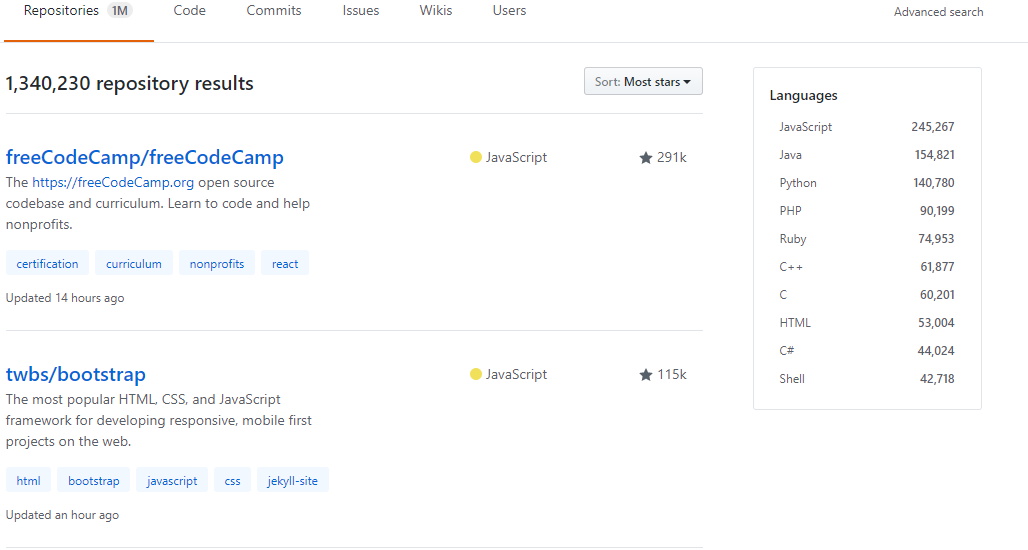
\includegraphics[width=1\textwidth]{Boostrap_statics_github.png}
		\caption{Bootstrap second starred on github}
	\end{figure}
	
	\vspace{66mm}
	
	According to a researchs, did it by myself in the net, all the high-tech blogs encourage developers to use bootstrap.
	\\
	\\
	I used a tool offred by google named \textbf{google trends} to make a compraison between a subjects in term of most researched.
	\\
	After this compraison in google trends, Bootstrap also is the most googled css framework on the web , compared to the others css frameworks Eg. \textbf{Foundation} which was considered as the most popular css framework after Boostrap.
	\begin{figure}[h]
		\centering
		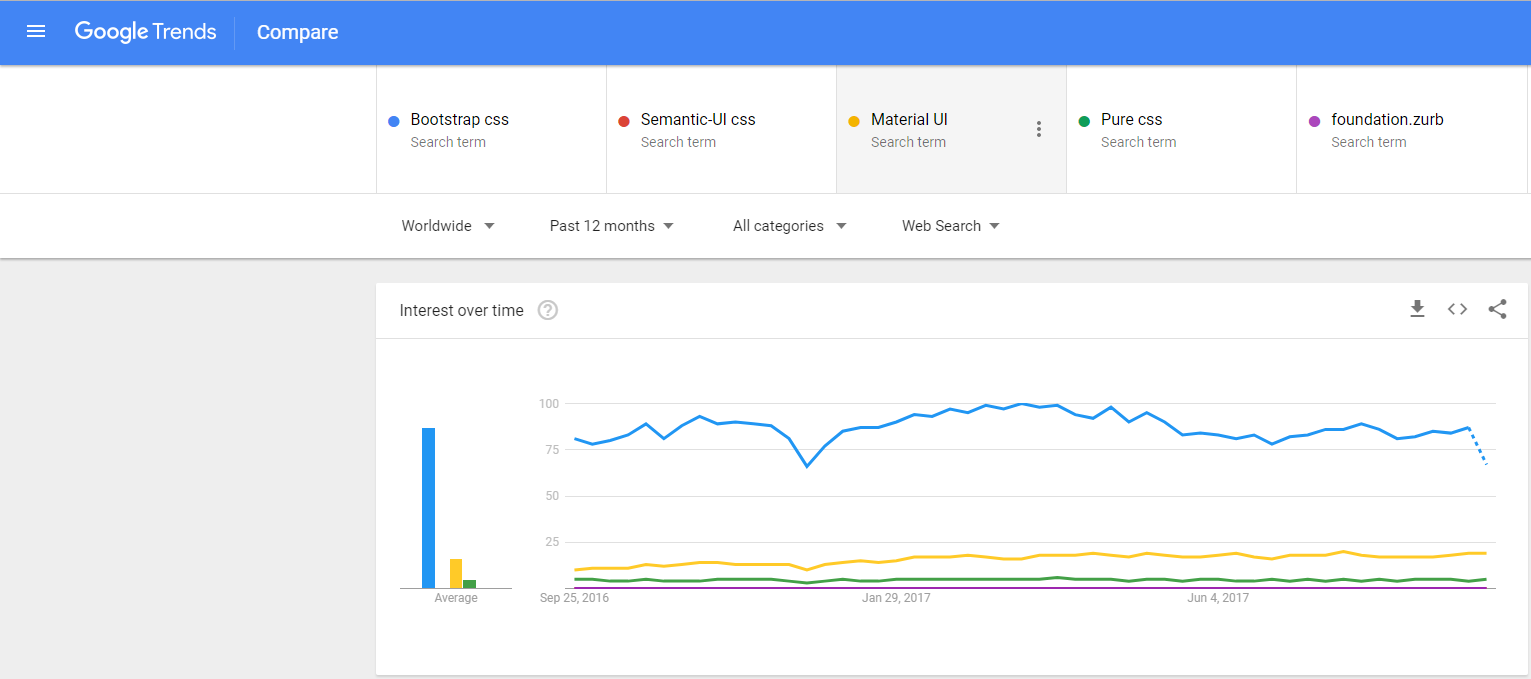
\includegraphics[width=1\textwidth]{Boostrap_statics_google_trends.png}
		\caption{Bootstrap on google trends}
	\end{figure}
\end{document}